% !TEX root = ../paper.tex
\begingroup
\makeatletter
\setlength{\@fptop}{0pt}
\setlength{\@fpsep}{12pt}
\makeatother
\section{Dataset Distribution and Additional Visual Evidence}
\label{sec:visual_details}
\setcounter{figure}{0}
\renewcommand{\thefigure}{B.\arabic{figure}}

Figure~\ref{fig:dataset_details} reports per-scene counts and acquisition attributes.
Figures~\ref{fig:additional_product} and \ref{fig:night_control}
extend the main-text examples to a tower-orbit sequence and the night zoom/wide control.
All displays use frozen estimates and the same image crops as the corresponding source records.

\begin{figure}[!htbp]
\centering
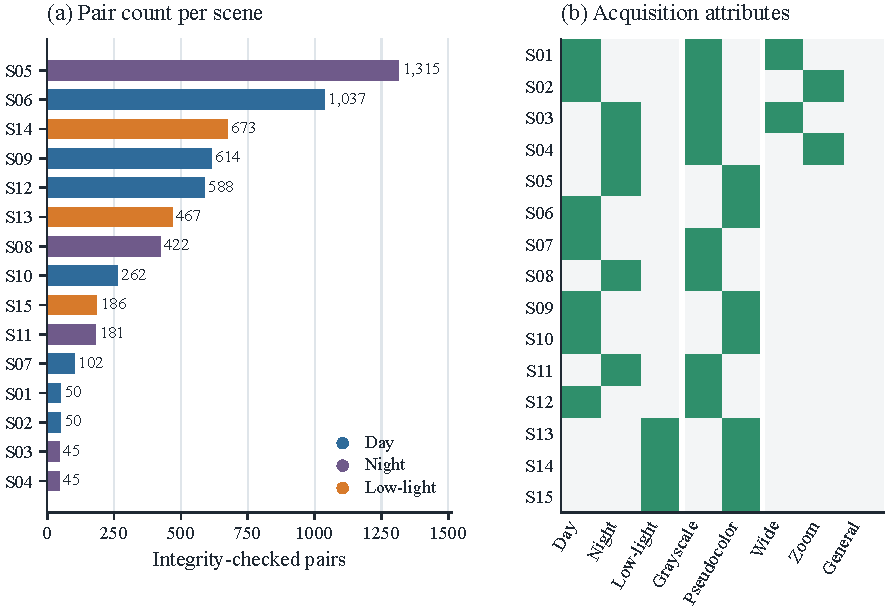
\includegraphics[width=\textwidth]{figures/fig02_dataset_details.pdf}
\caption{Official evaluation split: (a) valid pair counts and (b) acquisition attributes of
the 15 scenes. Color in (a) identifies illumination; filled cells in (b) identify scene attributes.}
\label{fig:dataset_details}

\vspace{10pt}
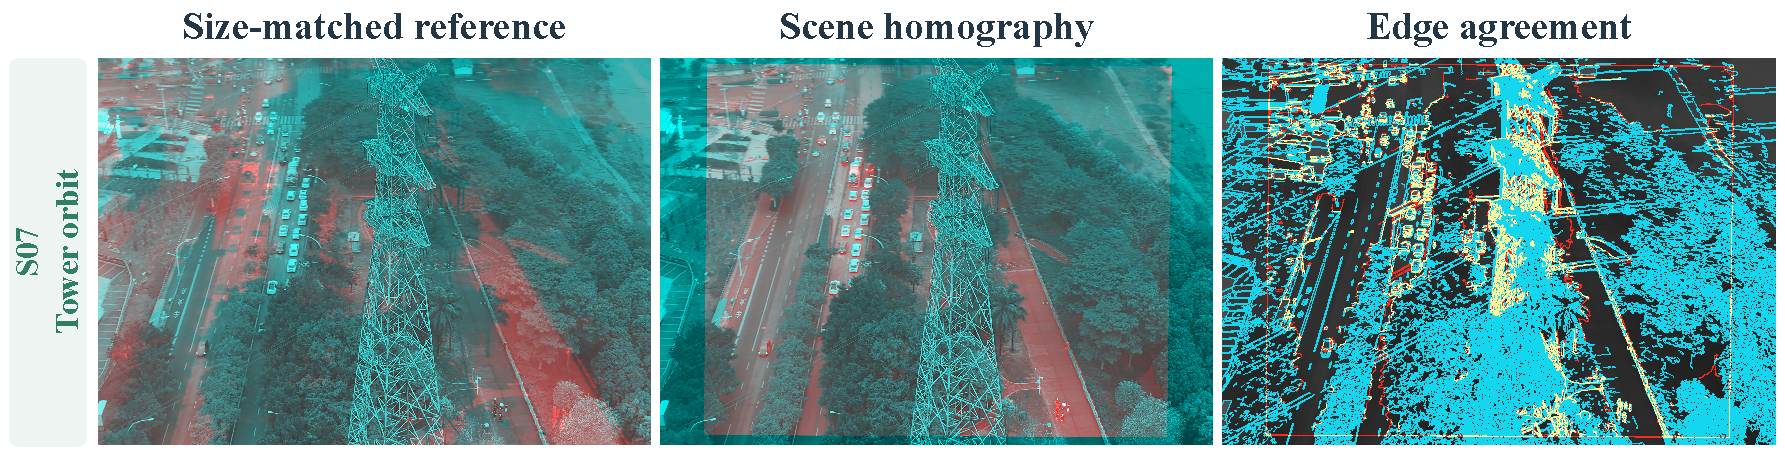
\includegraphics[width=\textwidth]{figures/fig06_additional_product.pdf}
\caption{Additional canonical product from the S07 tower-orbit sequence. The panels compare
the size-matched reference, scene-homography overlay, and edge agreement on the same display crop.}
\label{fig:additional_product}
\end{figure}

\begin{figure}[!htbp]
\centering
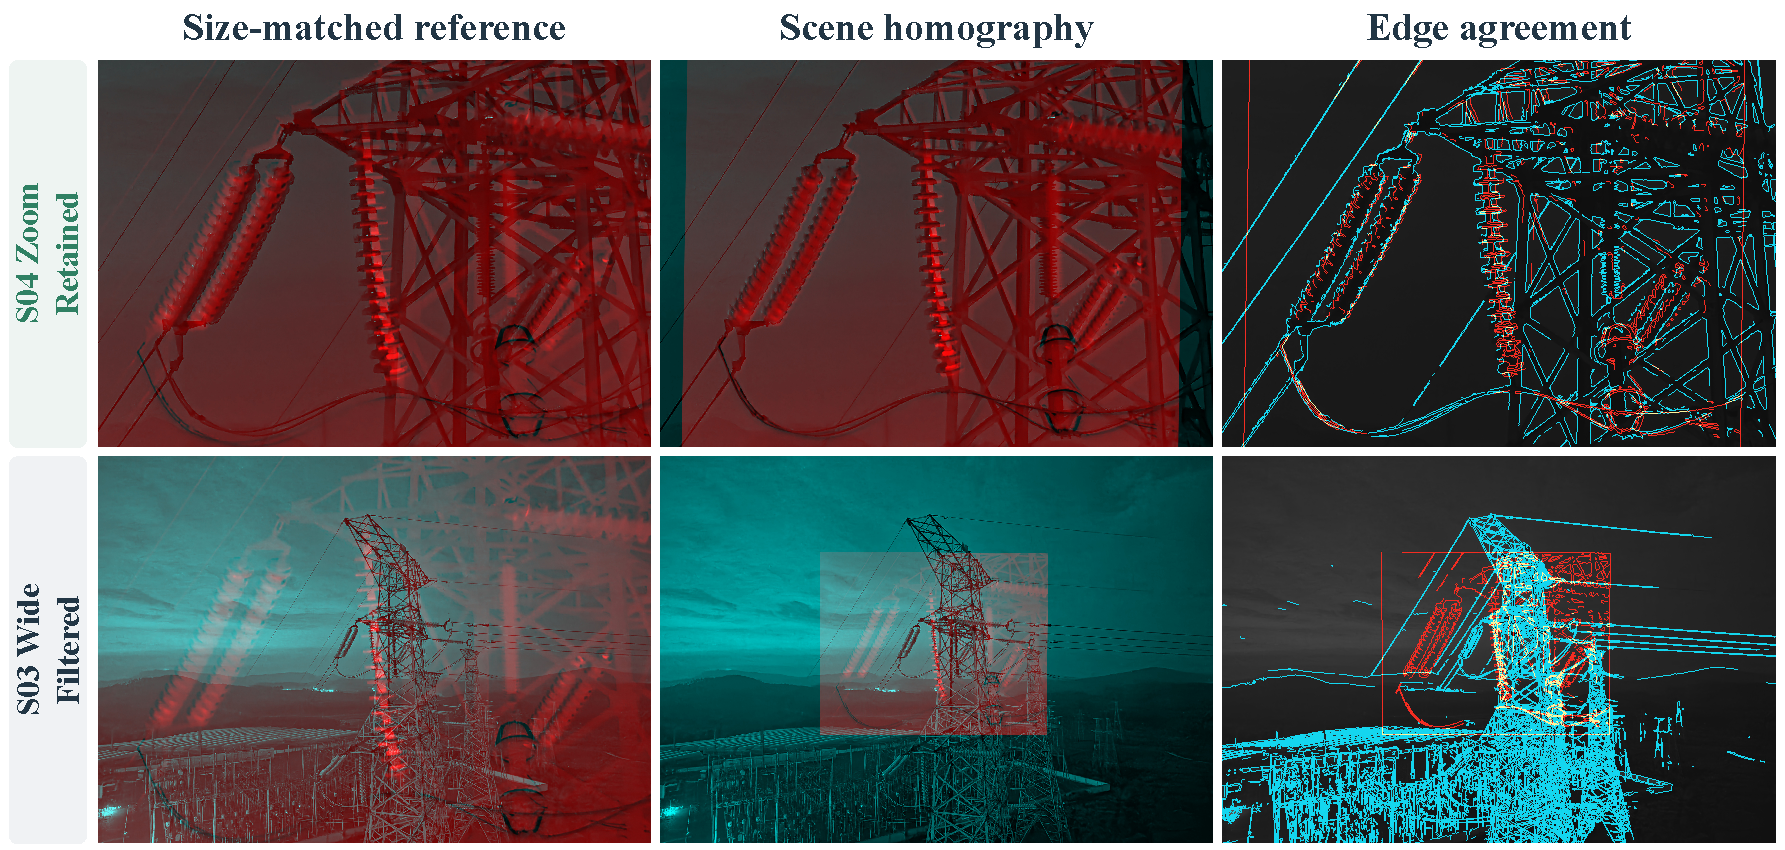
\includegraphics[width=\textwidth]{figures/fig07_night_control.pdf}
\caption{Night zoom/wide control. S04 is canonically retained and S03 is QA-filtered.
Each row shows the size-matched reference, estimated scene homography, and edge agreement.
The filtered estimate remains visible for inspection.}
\label{fig:night_control}

\vspace{10pt}
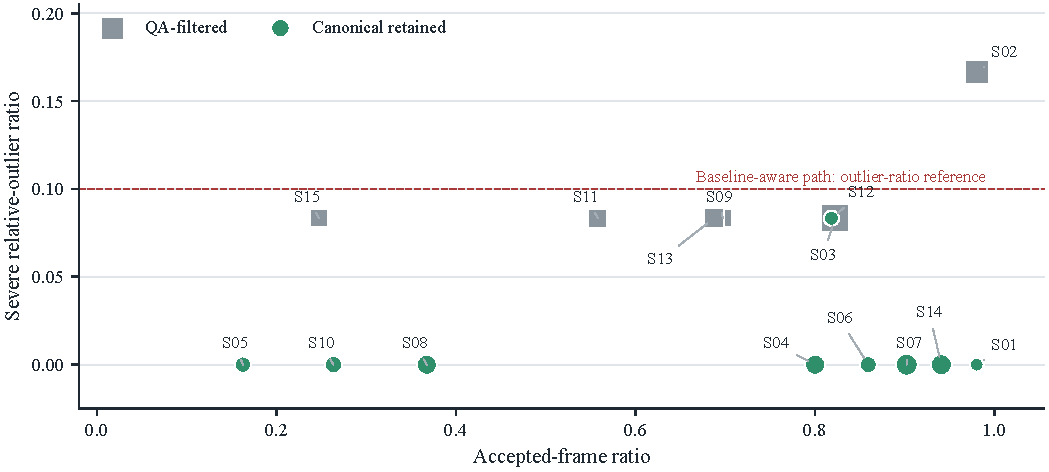
\includegraphics[width=\textwidth]{figures/fig07_qa_scatter.pdf}
\caption{All-scene QA diagnostics. Circles denote canonical retained scenes and squares denote
QA-filtered scenes; marker size represents robust-rejection ratio. The dashed line marks the
0.10 severe-outlier-ratio reference used in the baseline-aware path. The full canonical decision
combines the verification paths and support requirement in \ref{sec:canonical_details}.}
\label{fig:all_scene_qa}
\end{figure}
\FloatBarrier
\endgroup
